\section{Null space cardinality}
In the first lecture, we defined 4 spaces: $N(A), N(A^\intercal), \mathcal{C}(A), \mathcal{C}(A^\intercal)$. For the last two we defined also their cardinality whilst for the first ones we weren't able to tell yet. In this lecture we are going to find those values and prove them. In order to do so, we start from few useful properties:
\begin{enumerate}
    \item $\underline{x} = \underline{0} \in N(A)$ for any matrix $A$
    \item if $\underline{x}, \underline{y} \in N(A) \implies A(\underline{x} + \underline{y}) = \underline{0}$
    \item if $\underline{x} \in N(A) \implies \alpha\underline{x}$ with $\alpha \in \mathbb{R} \implies A(\alpha\underline{x}) = \underline{0}$
\end{enumerate}  

Consider, once again, the matrix $A \in \mathbb{R}^{m\times n}$, rank($A$) = $r \leq n$. 
We have seen the decomposition $A = CR$, where $C$ contains the linearly independent columns of $A$ and $R$ contains the coefficients that allow to recover the columns of $A$ starting from its independent columns. 
So, the matrix $A$ can be rewritten as:
\[
  A = \begin{bmatrix}
    A_1 & A_2
  \end{bmatrix} 
  \hspace{1cm}
  A_1 \in \mathbb{R}^{m\times r} \hspace{1cm} A_2 \in \mathbb{R}^{m\times (n-r)} 
\]
Where $A_1$ contains the independent columns of $A$ and $A_2$ the dependent ones.
Example:
\[
A = 
\begin{bmatrix}
    1 & 4 & 7\\
    2 & 5 & 8\\
    3 & 6 & 9
\end{bmatrix}
= 
\underbrace{
\begin{bmatrix}
1 & 4\\
2 & 5\\
3 & 6
\end{bmatrix}}_{A_1}
\begin{bmatrix}
    1 & 0 & -1\\
    0 & 1 & \undermat{B}{2}
\end{bmatrix}
\]
Since we have the last column of $A$, that is linearly dependent so it belongs to $A_2$, we can reformulate it in this way:
\[
    A = \begin{bmatrix}
        A_1 & A_2
      \end{bmatrix} 
    = \begin{bmatrix}
        A_1 & A_1B
    \end{bmatrix}
\]
We build a new matrix $K$ defined as follows:
\[
    K = \begin{bmatrix}
        -B\\
        I_{n-r}
    \end{bmatrix}
    \hspace{1cm}
    K \in \mathbb{R}^{n\times(n-r)}    
    \hspace{1cm}
    B \in \mathbb{R}^{r\times(n-r)}    
\]

\[
AK = \begin{bmatrix}
    A_1 & A_1B
\end{bmatrix} 
\begin{bmatrix}
    -B\\
    I_{n-r}
\end{bmatrix}
= A_1(-B) + A_1B = 0   
\]
Where the last 0 is actually a matrix of zeros of dimension $m\times(n-r)$
because A has size $m\times n$ and $K$ has size $n\times(n-r)$.
We have that:
\[
    AK = 0 \implies A\underline{k_i} = 0 \hspace{1cm} \forall i \in \{1, \dots, n-r\}    
\]
Where $k_i$ is the i-th column of $K$. This means that: $\underline{k_i} \in N(A) \hspace{0.2cm} \forall i$.

Now, we want to demonstrate that: $K\underline{u} = 0 \implies \underline{u} = \underline{0}$. 
To do so, we start from expanding $K$ from its definition:
\[
    K = \begin{bmatrix}
        -B\\
        I
    \end{bmatrix}
    \underline{u} = 0
    \implies
    \begin{bmatrix}
        -B\underline{u}\\
        \underline{u}
    \end{bmatrix}
    = 
    \begin{bmatrix}
        \underline{0}\\
        \underline{0}
    \end{bmatrix}
\]
Where the two zero vectors have dimension $r$ and $n-r$ respectively! Considering the second row of the matrix we get: $\underline{u} = \underline{0}$ so all columns of $K$ are linearly independent.\\

If we consider the problem ($\star$) $A\underline{x} = \underline{0}$, we want to prove that each \underline{x} that satisfy ($\star$) must be a linear combination of the columns of $K$.\\
\[
    A_1\underline{x} = \underline{0} \in \mathbb{R}^m \implies \underline{x} = \underline{0} \in \mathbb{R}^r    
\]
Because $A_1$ has linearly independent columns, i.e. has full rank.
\[
    A\underline{u} = \underline{0} \in \mathbb{R}^m \implies \begin{bmatrix}
        A_1 & A_1B
    \end{bmatrix} 
    \begin{bmatrix}
        \underline{u_1}\\
        \underline{u_2}
    \end{bmatrix}  
    = 
    \begin{bmatrix}
        A_1\underline{u_1} + A_1B\underline{u_2}\\
    \end{bmatrix}
    = 
    A_1\left[\underline{u_1} + B\underline{u_2}\right]
    = \underline{0}
\]
We can notice that the last formulation obtained in the equation has the same form as the one from where we started the prove, so we can say that:
\[
    \underline{u_1} + B\underline{u_2} = \underline{0} \implies \underline{u_1} = -B\underline{u_2}    
\]
\[
   \underline{u} = \begin{bmatrix}
    -B\underline{u_2}\\
    \underline{u_2}
\end{bmatrix}
    =
\underbrace{\begin{bmatrix}
    -B\\
    I
\end{bmatrix}}_{K}
    \underline{u_2}
    = K\underline{u_2}
    \implies 
    dim(N(A)) = n - r
\]


\begin{center}
    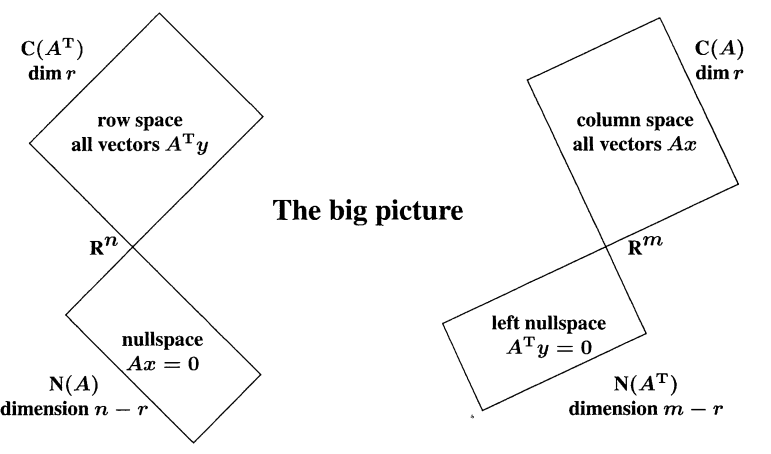
\includegraphics[scale = 0.4]{../images/SpacesDimensions.png}
\end{center}


\section{Eigenvalues and eigenvectors}
Start considering a generic square matrix $n \times n$. We are going later to discuss even the simmetry and positive definite properties.
Here below are the vectorial and the matrix form of the eigenvalue problem:
\[
    A\underline{x_i} = \lambda_i\underline{x_i} \hspace{0.5cm} i = 1, \dots, n \hspace{1cm} X^{-1}AX = \Lambda
\]
Where in the right-hand side there is a diagonal matrix $\Lambda$ with the eigenvalues of $A$ on the diagonal while the matrix $X$ with the eigenvectors of $A$ as columns.\\

\subsection{Eigenvectors of matrix power}
What can we say about the eigenvectors and eigenvalues of $A^2$?
\[
    A^2\underline{x_i} = A(A\underline{x_i}) = A(\lambda_i\underline{x_i}) = \lambda_i(A\underline{x_i}) = \lambda_i^2\underline{x_i}    
\]
So the eigenvalues of $A^2$ are the eigenvalues of $A$ squared.This is valid for any power of $A$ since this method can be applied recursively and it is very useful when there are problems in which a matrix is iteratively multiplied many times. \\

\textbf{Important}:\\
Given $A\in \mathbb{R}^{n\times n}$ full rank, then any vector $\underline{v} \in \mathbb{R}^n$ can be written as a linear combination of the eigenvectors ($x_i$) of $A$.\\

\subsection{Power method}
In mathematics, power iteration (also known as the power method) is an eigenvalue algorithm: given a diagonalizable matrix A, the algorithm will produce a number $\lambda$ , which is the greatest (in absolute value) eigenvalue of A, and a nonzero vector v, which is a corresponding eigenvector of $\lambda$ , that is, $Av=\lambda v$. The algorithm is also known as the Von Mises iteration.

There is also an \textbf{inverse PM} which is applied to $A^{-1}$ to find the minimum eigenvalue or also \textbf{PM with a shift} applied to $(A-\alpha I)^{-1}, \alpha \in \mathbb{R}$ to find the closest eigenvalue to $\alpha$. 

Can even be used in "deflation method" iteratively:
\[
    \begin{bmatrix}
        \lambda_1 & \underline{b_1^\intercal}\\
        0 & A_1
    \end{bmatrix}    
\]
the original matrix could be reduced in that form and at every iteration the procedure is applied to the $A_1$ matrix. This works only if we have different eigenvectors (or values) [check].

\subsection{Similar matrices}
Given two matrices $A, B \in \mathbb{R}^n$, they are said to be similar if $B = M^{-1}AM$, with $M$ invertible. 
\[
    \underbrace{M^{-1}AM}_{B}\underline{y} = \lambda \underline{y} \implies A\underbrace{M\underline{y}}_{\underline{w}} = \lambda \underbrace{M\underline{y}}_{\underline{w}} = A\underline{w} = \lambda \underline{w}    
\]
Where $\lambda, \underline{y}$ contain respectively the eigenvalues and the eigenvectors of $B$. What we get from this equation is that \textbf{similar matrices share the same eigenvectors with scaled eigenvalues}.

\subsection{QR factorization}
Here is introduced in the context of eigenvalues. Let's consider a matrix $A \in \mathbb{R}^{m\times n}$ where $m \geq n$ and $rank(A) = n$ (it has all independent columns). We can factorize $A$ in this way:
\[
    A = QR \hspace{1cm} Q \in \mathbb{R}^{m\times n} \hspace{1cm} R \in \mathbb{R}^{n\times n}
\]
Where is $Q$ is an orthogonal matrix and $R$ is an upper triangular matrix.Since we are dealing with eigenvalues and eigenvectors, we are now going to consider the matrix $A$ squared with the dimension $n\times n$.

\subsubsection{QR iteration} 
\[
    A = A^{(0)} = Q^{(0)}R^{(0)}     
\]
\[
    A^{(1)} = {Q^{(0)}}^{\intercal} A^{(0)} Q^{(0)} = Q^{(1)} R^{(1)}    
\]
So, iterating this procedure we get:
\[
    A^{(2)}, \dots, A^{(S)} = \text{is upper triangular}
\]
After S iterations you obtain an upper triangular matrix. The matrices $A, A^{(0)}, A^{(1)}, \dots, A^{(S)}$ are similar, so they share the same eigenvalues.

But, how can i compute $Q$?\\
With the \textbf{Gram-Schmidt} procedure. It works also for non-square matrices.\\
Let's start from a generic matrix $A$:
\[
    A = \begin{bmatrix}
        \vline & \vline & \vline\\
        \underline{a_1} & \ldots & \underline{a_n}\\
        \vline & \vline & \vline
    \end{bmatrix} 
\]
The algorithm is iterative and it is applied to the columns of $A$ in such way:
\[
  \underline{q_1} = \frac{\underline{a_1}}{||\underline{a_1}||}  
\]
The vector $\underline{q_1}$ is obtained by normalizing the first column of $A$, in such manner the new obtained vector will have norm 1.
\[
    \underline{q_2} = \underline{a_2} - \underline{q_1}(\underline{q_1}^\intercal \underline{a_2}) \implies \underline{q_2} = \dfrac{\underline{q_2}}{||\underline{q_2}||}
\]
The second vector is obtained by subtracting from the second column of $A$ the projection of $\underline{a_2}$ on $\underline{q_1}$, in such manner the new vector will be orthogonal to $\underline{q_1}$ and will have norm 1.
\[
    \underline{q_3} = \underline{a_3} - \underline{q_1}(\underline{q_1}^\intercal \underline{a_3}) - \underline{q_2}(\underline{q_2}^\intercal \underline{a_3}) \implies \underline{q_3} = \dfrac{\underline{q_3}}{||\underline{q_3}||}
\]
And so on... Recall that the orthogonality is needed since we want to obtain an orthogonal matrix $Q$ useful for the factorization. With Gram-Schmidt the resulting matrix not only will be orthogonal but also orthonormal, this means that its columns will have norm unitary.\\  